\section{Interpreter}
\label{InterpreterIntro}
Der folgende Abschnitt beschäftigt sich mit dem Aufbau und der Funktionsweise des Interpreters. Die Aufgabe des Interpreters ist es anhand der vom \underline{Parser} erzeugten Datenstrukturen, den sogenannten Knoten (englisch: Nodes), die Semantik der Sprache korrekt zu implementieren und auszuführen. Dafür sind insbesondere zwei Klassen von Bedeutung, welche in \ref{Interpretation} und \ref{Node} vorgestellt werden.

\subsection{Die Klasse Interpretation}
\label{Interpretation}
Zuerst wird die essentielle Funktionsweise der Klasse Interpretation geklärt da diese für das Vorgehen des Interpreters wichtig ist.
Diese Klasse besitzt folgende Attribute:

\begin{lstlisting}[caption=Attribute der Klasse Interpretation, language=Java]
private Interpretation parent;
private HashMap<String, Object> environment;
private int nestingLevel;
\end{lstlisting}
Das \textbf{nestingLevel} wird hauptsächlich für die Annotatierbarkeit von Daten in einer Schleife benötigt, um das korrekte zu annotierende Datum in jeder Iteration zu bestimmen. Dies hängt eng mit dem sogenannten \textit{mapValue} zusammen, einer speziellen sprach-internen Variablen, welche für Schleifen benötigt wird. Da dies aber mehr mit der Sprache und ihren Konstrukten an sich zusammenhängt wird es hier nicht weiter konkretisiert. Für eine detaillierte Ausführung sei an die Sprachbeschreibung verwiesen.
\\\\
Das wohl wichtigste Attribut ist das hier genannte \textbf{environment}. Hier wird zur Laufzeit die Variablenbelegung des Programms festgehalten. Eine Zuweisung fügt dem \textbf{environment} somit entweder ein neues Schlüssel-Wert-Paar hinzu oder verändert den Wert eines bereits vorhandenen Schlüssels.

Da die Sprache Blöcke, Verschachtelungen und auch Funktionsaufrufe erlaubt, welche jeweils eine eigene Variablenbelegung besitzen können, wird eine Möglichkeit benötigt den Sichtbarkeitsbereich einer Variablen bzw. \textbf{environments}  zu beeinflussen. Dies wird durch das \textbf{parent}-Attribut realisiert. Bei jedem Aufruf eines neuen Blocks durch z. B. einer \textit{if-Anweisung}, einer \textit{for-Schleife} oder eines \textit{Funktionsaufrufs} wird eine neue Interpretation (mit leerem \textbf{environment}) erzeugt und die aktuelle Interpretation als \textbf{parent} gespeichert. Dies ermöglicht einem Block sowohl auf die Variablen der höheren Ebene(n) zuzugreifen als auch eigene lokale Variablen anzulegen welche am Ende des Blocks wieder verschwinden. 

Zudem können temporäre Interpretationen erzeugt werden, welche Zugriff auf die tatsächliche Variablenbelegung haben und dadurch bestimmte Sprachkonstrukte evaluieren können. 

Diese zwei Attribute \textbf{environment} und \textbf{parent} sind somit von zentraler Bedeutung bei der Verarbeitung und Speicherung von Variablen während der Evaluierung der vom \underline{Parser} erzeugten Datenstrukturen.
Es sollte hierbei erwähnt werden dass zu Beginn das Environment der ersten Interpretation mit den vorgefertigten Methoden aus der \underline{Standardbibliothek} befüllt wird um dem Nutzer vorab einige Funktionalitäten zur Verfügung zu stellen.


\subsection{Die Klasse Node}
\label{Node}
Bei den Datenstrukturen handelt es sich um Objekte der Klasse \textbf{Node}, genauer gesagt um die vielen Klassen welche von \textbf{Node} erben und in Baumstruktur vom \underline{Parser} bereitgestellt werden. Diese hierarchische Strukur bedeutet dass bis auf die Blätter jedes Objekt dieser Knoten weitere Knoten als Attribute hält. Jede (nicht-abstrakte) von \textbf{Node} abgeleitete Klasse implementiert folgende Methode:


\begin{lstlisting}[caption=Funktionsdeklaration der Methode \textit{evaluateNode}, language=Java]
public Object evaluateNode(Interpretation interpretation);
\end{lstlisting}
Die Funktionsweise von \textit{evaluateNode} kann grob in zwei Kategorien gliedern werden, je nachdem welche Art von Knoten sie aufruft:
\begin{itemize}
  \item Blattknoten: Gibt den Wert zurück, welcher von dem \underline{Parser} in diesem Knoten gespeichert wurde.
  \item Nicht-Blattknoten: Ruft zuerst die \textit{evaluateNode}-Methode aller der in dem Knoten gespeicherten Knoten auf und führt dann mit deren Rückgabewerten eine Operation aus.
\end{itemize}
Das Verfahren entspricht einer Art Tiefensuche beginnend mit dem Wurzelknoten bei der zuerst ein Pfad bis zu einem Blattknoten beschritten wird, welcher anschließend ein Rückgabewert an den "oberen" Knoten gibt. Hat ein Knoten alle Ergebnisse seiner Knoten erhalten wird eine Operation durchgeführt, welche von der jeweiligen Klasse abhängt. So enthält z.B. die Klasse \textbf{AddNode} zwei weitere Knoten als Attribute, dessen evaluierte Ergebnisse sie addiert.


Auf diese Weise wird Schritt für Schritt der vom Programmierer geschriebene Code ausgeführt indem der \underline{Parser} zu jedem Statement einen Syntaxbaum erzeugt welcher anschließend interpretiert wird.

\begin{figure}[H]
\centering
	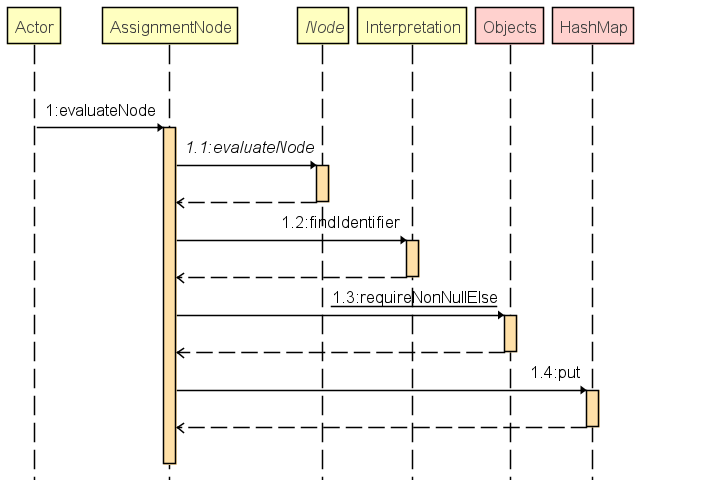
\includegraphics[width=1.1\textwidth]{images/AssignmentSequenz.png}\par\vspace{0.5cm}
	\caption{Sequenzdiagramm einer Zuweisung wie z.B. 'a := 5;'}
	\label{fig:sequence-assignment}
\end{figure}

Die oben aufgeführte Abbildung \ref{fig:sequence-assignment} zeigt den Evaluationsablauf eines Zuweisung-Statements. Ein \textbf{AssignmentNode} enthält einen weiteren Knoten, welcher zuerst evaluiert wird. Der Rückgabewert ist der zuzuweisende Wert. Als Nächstes muss geprüft werden ob der zu verwendende Identifikator bereits in einer Interpretation in Verwendung ist. Dafür wird die Methode \textit{findIdentifier} aufgerufen, welche in der aktuellen und rekursiv allen \textbf{parent} Interpretationen danach sucht. Wurde eine Interpretation gefunden, so wird der zuzuweisende Wert an die Stelle des Identifikator-Schlüssels in das \textbf{environment} geschrieben, andernfalls wird ein neues Schlüssel-Wert-Paar in das aktuelle \textbf{environment} gelegt.
\\\\
Zwischen der Klasse \textbf{Node} und den angeleiteten Klassen welche direkt vom Interpreter evaluiert werden bestehen weitere Ebenen von Knoten. Diese wurden hauptsächlich eingebaut um eine sinnvolle Gruppierung der Funktionalität zu gewährleisten und zur Reduzierung von mehrfach dupliziertem Code. So ist z.B. \textbf{BinaryArithmeticNode} eine von \textbf{ArithmeticNode} abgeleitete Klasse welche wiederum von \textbf{Node} erbt. Alle Knoten, welche für die Evaluierung von binären arithmetischen Operationen ('+', '-', '*' usw.) zuständig sind, leiten schlussendlich von dieser Klasse ab.

Durch diese Struktur kann der Interpreter in Zukunft leicht um Methoden erweitert werden, die nur von bestimmten Knoten ausgeführt werden sollen. 
Insgesamt können vom \underline{Parser} über 60 verschiedene solcher von \textbf{Node} abgeleiteten Klassen erzeugen um alle Sprachkonstrukte abzudecken und welche vom Interpreter evaluiert werden müssen. Das folgende Klassendiagramm soll zur Veranschaulichung der groben Struktur dienen. 
\begin{figure}[H]
\centering
	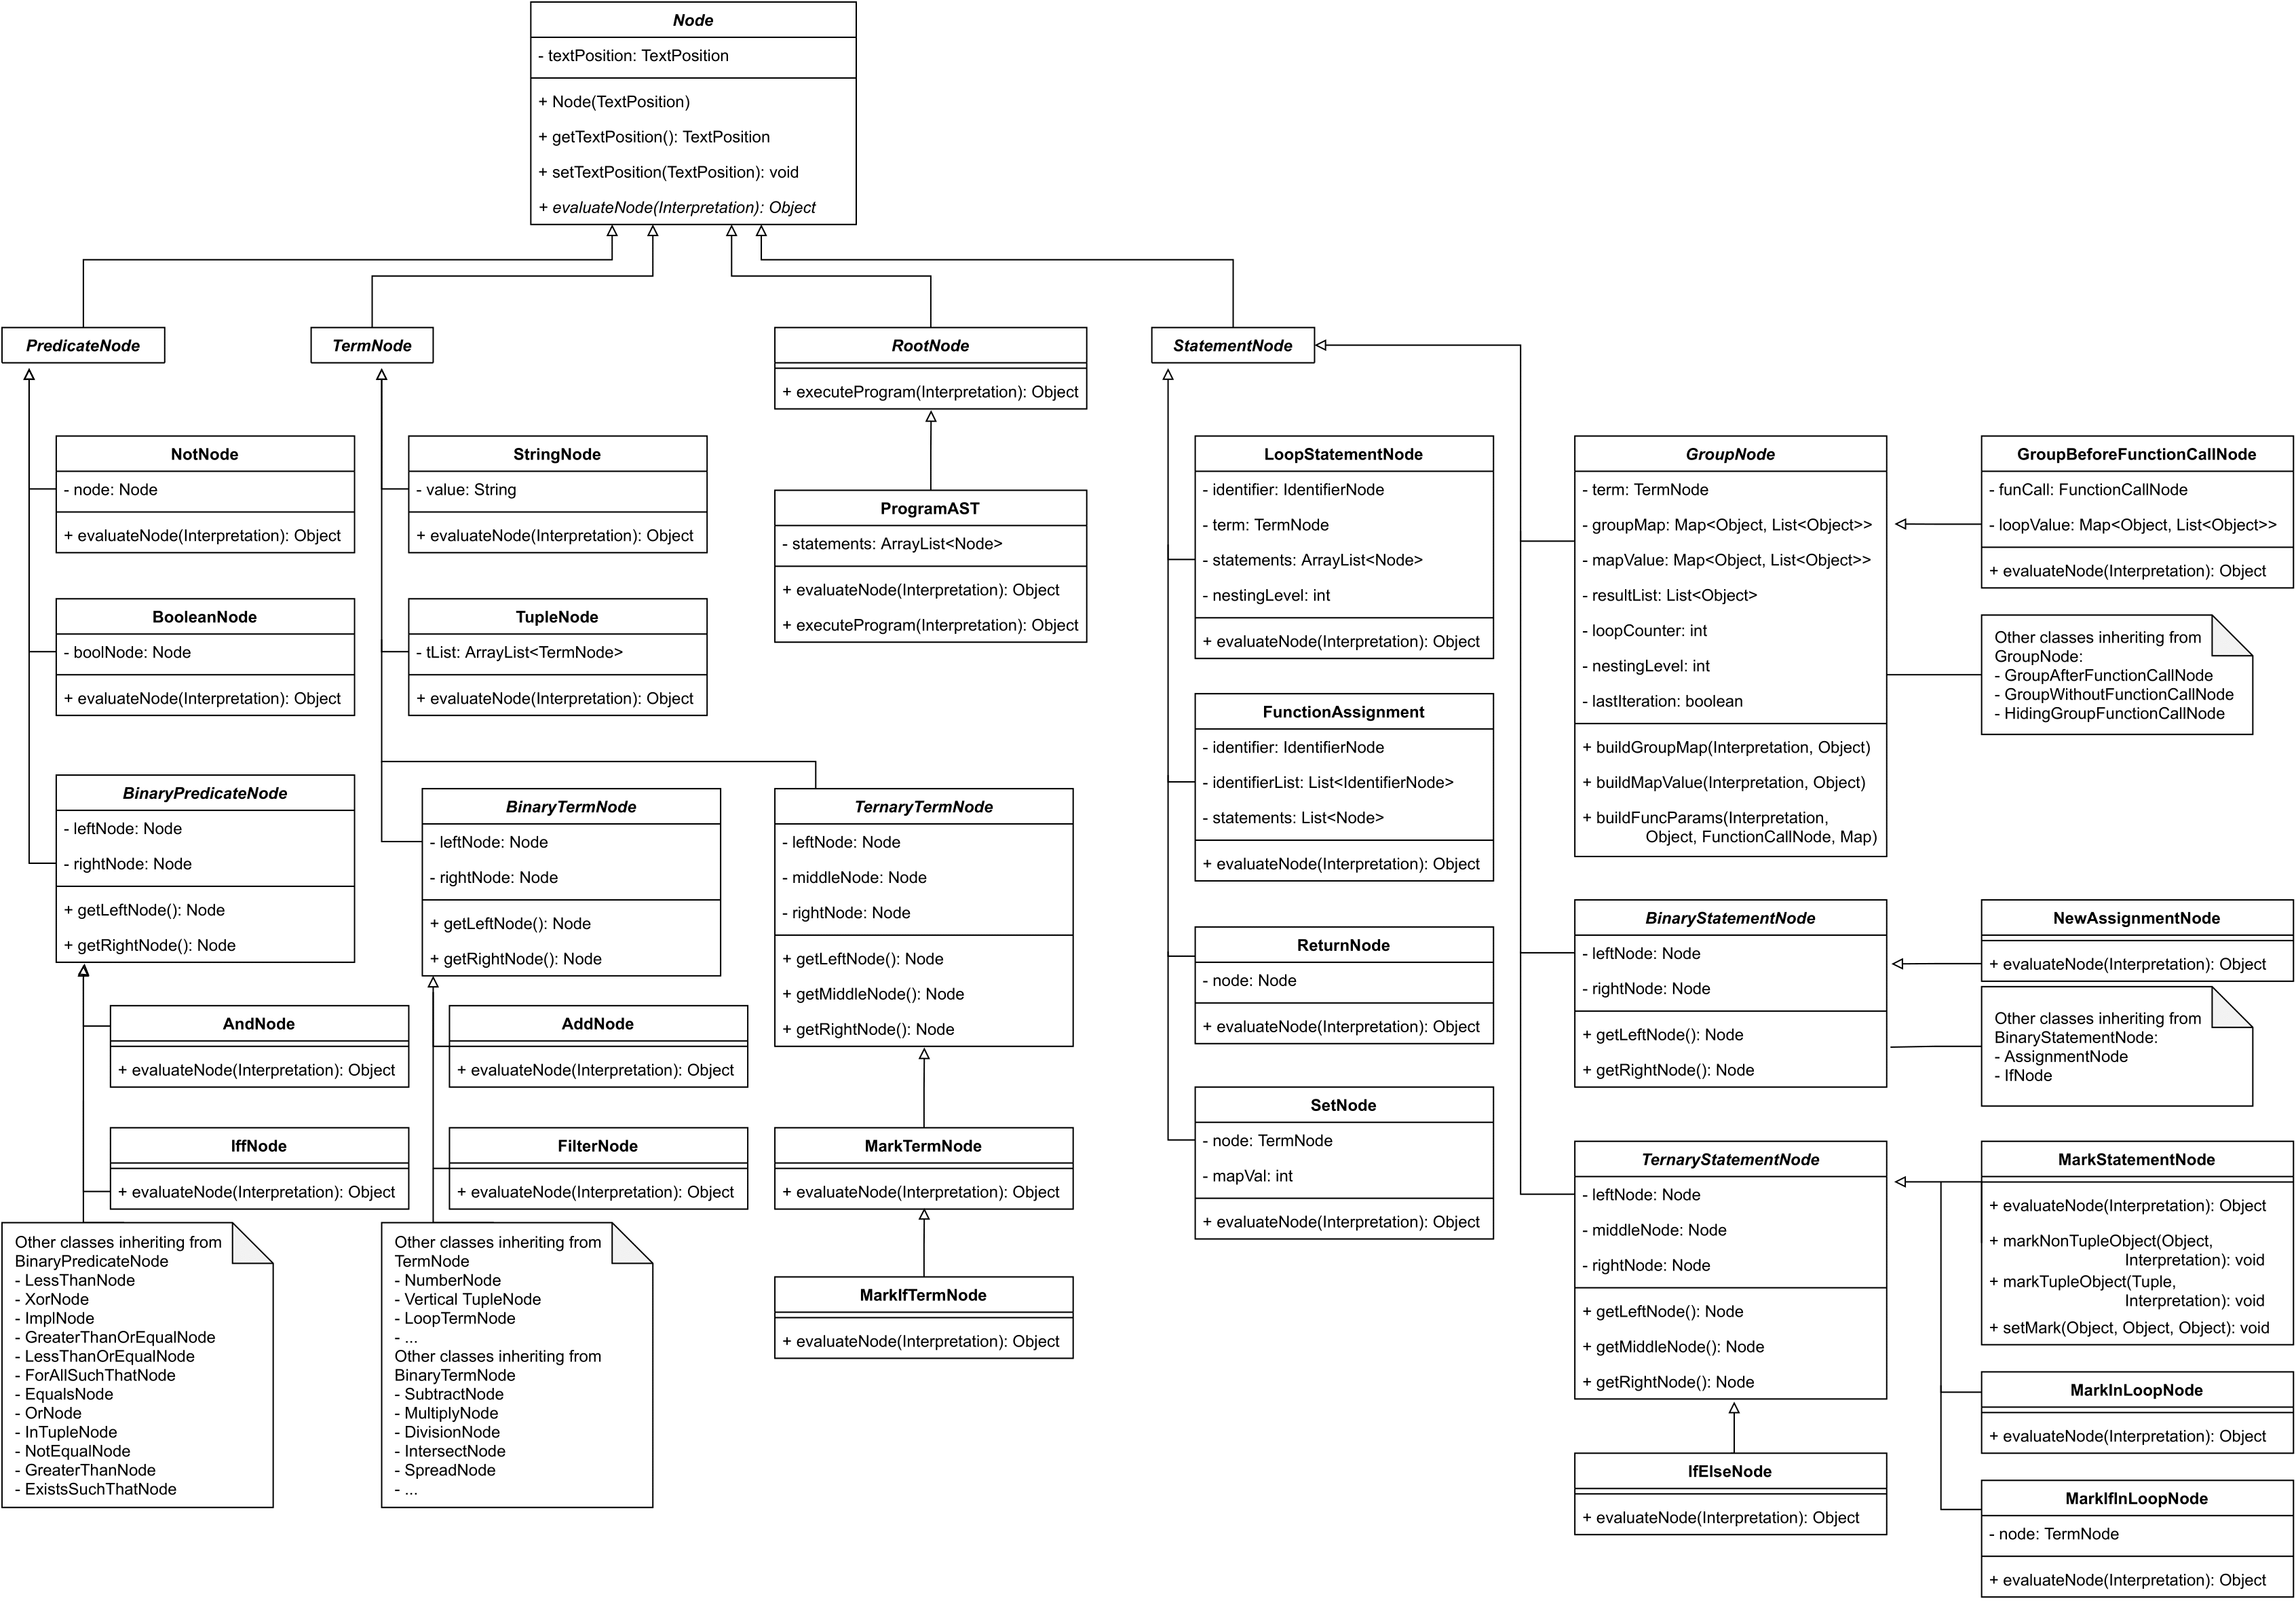
\includegraphics[width=1.1\textwidth]{images/NodeClassDiagram-1.png}\par\vspace{0.5cm}
	\caption{Klassendiagramm - Node}
\end{figure}

Es muss jedoch beachtet werden dass der \underline{Parser} nicht überprüft ob die Operanden einer Operation die korrekten \underline{Datentypen} besitzen. So kann es zur Laufzeit zu Fehlern kommen. Dies ist auch Aufgabe des Interpreters. Um dies zentral gebündelt an einer Stelle zu überprüfen enthält die Klasse \textbf{Node} zusätzlich folgende Methoden:

\begin{lstlisting}[caption=Methoden zur Typüberprüfung,label={lst:verifyMethods}, language=Java]
public Table verifyAndReturnTable(Interpretation in);
public InternalNumber verifyAndReturnNumber(Interpretation in);
public InternalBoolean verifyAndReturnBoolean(Interpretation in);
public InternalString verifyAndReturnString(Interpretation in);
public TupleOperation verifyAndReturnTupleOperation(Interpretation in);
\end{lstlisting}
Im Inneren der Funktion wird der Knoten der sie aufruft wie normal evaluiert, nur wird nach Berechnung des Ergebnisses geprüft ob dieses dem korrespondierenden \underline{Datentyp} entspricht. Wenn ja wird es zurückgegeben, wenn nicht wird eine Exception geworfen.

Jeder Knoten kann somit durch Aufruf einer dieser Methoden sicherstellen, dass die \underline{Datentypen} seiner Operanden korrekt sind. Beispiel: In einer \textbf{MultiplyNode} rufen beide Nachfolgerknoten die Methode \textit{verifyAndReturnNumber} auf um zu überprüfen dass deren Ergebnisse Zahlen sind bevor die Multiplikation ausgeführt wird. Ansonsten wird eine Fehlermeldung ausgegeben. 

Das folgende Sequenzdiagramm veranschaulicht eine korrekte Evaluierung einer \textbf{MultiplyNode}:
\begin{figure}[H]
\centering
	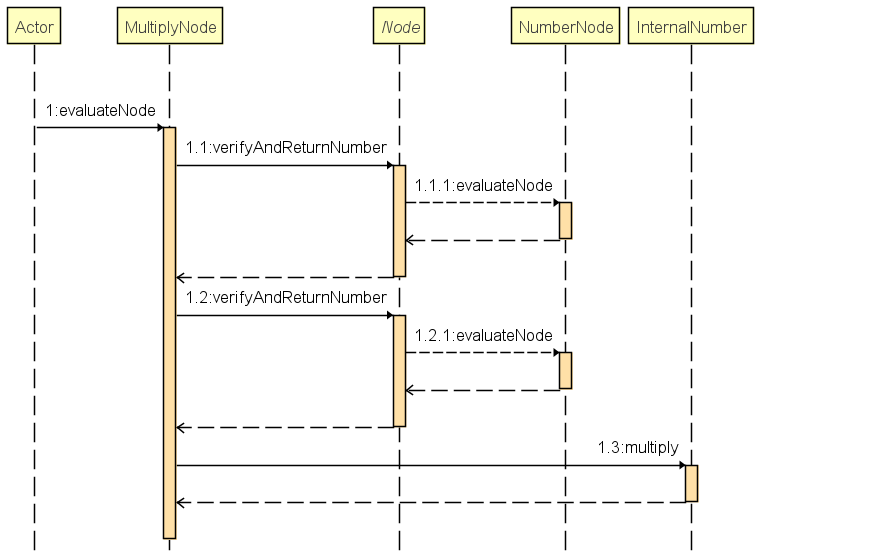
\includegraphics[width=1.1\textwidth]{images/MultiplySequenz.png}\par\vspace{0.5cm}
	\caption{Sequenzdiagramm - MultiplyNode}
\end{figure}


\subsection{Fehler während der Evaluierung}
\label{Fehlermeldungen}
Wie bereits erwähnt können zur Laufzeit des Interpreters Probleme auftreten, welche behandelt werden sollten. 
Falls während der Abarbeitung der Knoten ein Fehler auftritt, so wird eine Fehlermeldung ausgegeben. 

Um eine möglichst hilfreiche Meldung zu produzieren erhält jeder Knoten bei Erzeugung vom \underline{Parser} eine Textposition. Sollte nun bei der Ausführung der \textit{evaluateNode} eines Knotens ein Fehler auftreten, kann dem Nutzer anhand der Textposition gezeigt und markiert werden welche Zeile und Spalte des Quellcodes fehlgeschlagen ist. Des Weiteren kann jeder Knoten spezifische weitere Informationen bereitstellen weshalb eine Aktion nicht ausgeführt werden darf. Im Falle eines falschen \underline{Datentyps} werden zusätzlich die für die Operation erlaubten Operandentypen aufgelistet. Dies gilt auch für die in Listing \ref{lst:verifyMethods} aufgeführten Methoden.
